%% ==============================
\chapter{\iflanguage{ngerman}{Methoden}{Methods}}
\label{sec:methods}
%% ==============================


Diese Arbeit orientiert sich an dem zweistufigen Clusteringverfahren aus dem Paper von Nguyen \cite{nguyen2012clustering}. 
\newline
Zuerst müssen die LH-Werte des Volumen berechnet werden. Hierfür werden zunächst die Gradienten aller Voxel benötigt. Wie im Paper beschrieben wurde auch in dieser Arbeit Hong's Methode \cite{hong2003method} dafür gewählt.
Diese ist ein approximationsbasiertes Verfahren zur Berechnung von Gradienten eines Volumens. 
\newline
In Hong's Verfahren wird zur Berechnung der Gradienten die lokale 4x4x4 Nachbarschaft des betrachteten Punktes hinzugezogen. Hierbei ist zu beachten, dass es nicht möglich ist, den Gradienten für einen Voxel direkt zu berechnen. Der Gradient drückt die Veränderung der Intensitätswerte im Raum aus, folglich kann er immer nur zwischen zwei Punkten berechnet werden. Deshalb liegt er im Falle eines dreidimensionalen Volumens im Zentrum eins Würfels, der von 8 benachbarten Voxeln aufgespannt wird. In \autoref{fig:nachbarschaft} ist zu erkennen, wie der Gradient im Zentrum der acht Voxel liegt. Desweiteren ist die 4x4x4 Nachbarschaft in Form der durchnummerierten Punkte zu sehen.
\newline

\begin{figure}[!h] 
\centering 
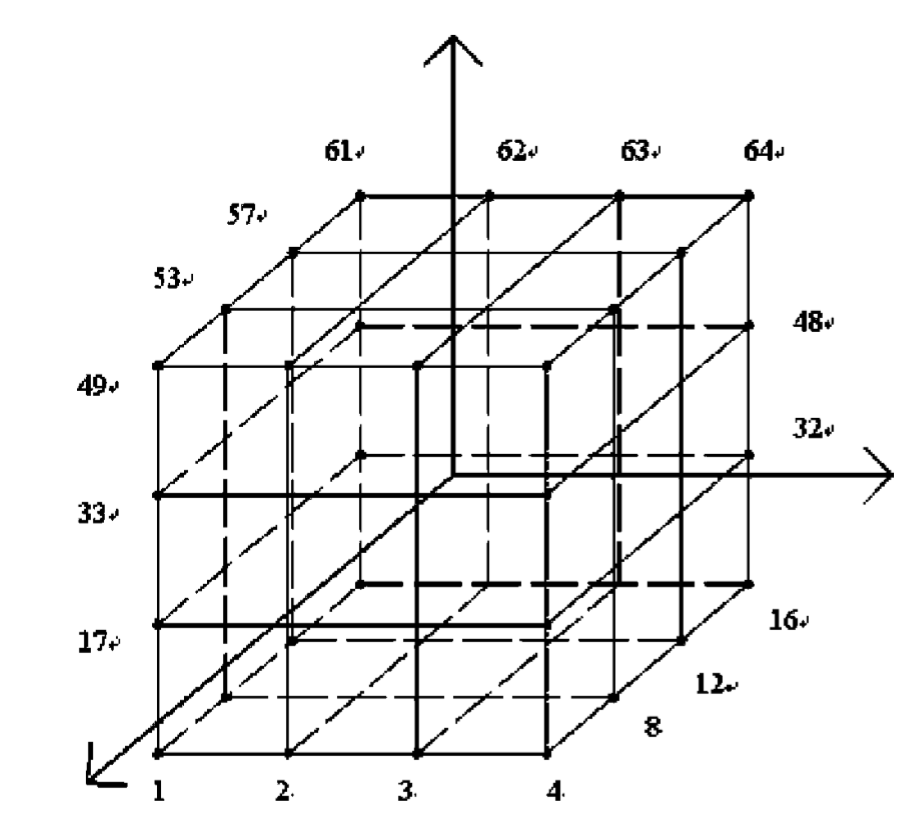
\includegraphics[width=\textwidth]{Logos/VoxelEdges.PNG}
\caption{Darstellung der lokalen 4x4x4 Nachbarschaft} 
\label{fig:nachbarschaft} 
\end{figure}
\todo{richtig bild zitieren u. evtl kleiner}

Die Funktionen für die Intensitätswerte wird im Paper mit:
\begin{equation}
	f(x,y,z) = Ax^{2}+By^{2}+Cz^{2}+2Fyz+2Gzx+2Hxy+2Ix+2Jy+2Kz+D
\end{equation}
approximiert. Da der Gradient die Ableitung der Intensitätsfunktion ist, erhält man den dreidimensionalen Gradientenvektor $n$, indem die Funktion ableitetet wird:
\begin{equation}
	n = (Ax+Gz+Hy+I, By+Fz+Hx+J, Cz + Fy + Gx + K)
\end{equation}
Um den Gradienten zu Berechnen müssen die Parameter $A,B,C,E,F,G,H,I,J,K$  berechnet werden. Dies geschieht mithilfe der Methode der kleinsten Quadrate.
\todo{methode der kleinsten quadrate genauer beschreiben}
\newline
Als nächster Schritt, nach der Kalkulation der Gradienten, folgt die Berechnung der Low- und High-Werte. Dazu wird in Richtung der Gradienten integriert. Hierfür wurde, wie auch von Nguyen, Heun's Methode, eine modifizierte Euler Methode, verwendet. Die für die Integration benutzte Formel lautet:
\begin{equation}
	u_{i+1} = u_{i} + \frac{1}{2}d(\triangledown f (u_{i}) + \triangledown f(u_{i}+d \triangledown f(u_{i}))) 
\end{equation}
Hierbei sind $u_{i}$ und $u_{i+1}$ die Positionen des aktuellen, beziehungsweise des nächsten Voxels. $\triangledown f(x)$ beschreibt den normalisierten Gradienten für die High-Werte und den normalisierten inversen Gradienten für die Low-Werte an Stelle $x$ . $d$ steht für die Schrittweite, die in dieser Arbeit auf einen Voxel festgelegt wurde.
Die Integration stoppt, wenn eine lokale Extremstelle oder ein Wendepunkt erreicht wird. Dies ist daran zu erkennen, dass die Länge des Gradienten an dieser Stelle null ist. Bei MRT-Daten muss ein Grenzwert festgelegt werden, da Gradienten nie null werden. Bei CT-Daten ist dies jedoch kein Problem. Wird ein solcher Punkt erreicht, wird der Intensitätswert dieses Voxels als Ergebnis für den Low- beziehungsweise High-Wert des Startvoxel gespeichert.
\newline
Anschließend wird ein LH-Histogramm mit allen berechneten LH-Wertpaaren erstellt. Hierbei sind auf der x-Achse die Low-Werte und auf der y-Achse die High-Werte angesiedelt. Die Werte der Achsen reichen von null bis zum jeweiligen Maximum des Low- beziehungsweise High-Werte.
\newline
Als nächstes, wird der erste Clusteringschritt berechnet. Dieser findet im LH-Raum statt, genauer wird er auf dem eben berechneten LH-Histogramm angewendet. Dabei kommt Meanshiftclustering zum Einsatz. Der Ablauf davon geschieht wie folgt.
Vor dem Clustering muss eine Bandweite und ein Thresholdwert bestimmt werden, welche die Sensitivität des Clusterings festlegen. Die Bandweite liegt im Paper von Nguyen \cite{nguyen2012clustering} bei 7\% - 9\% des maximalen LH-Wertes und der Threshold bei 0,01. Anschließend kann das LH-Clustering auf jeden Punkt im Histogramm angewandt werden.
\newline
Für einen beliebigen Punkt, werden alle Punkte die innerhalb des Radius der Bandbreite liegen gespeichert. Diese Punkte bilden nun den gefundenen Cluster. Von diesem Cluster wird der neue Mittelpunkt, der jeweilige Mittelwert der beiden Koordinaten, berechnet. Um diesen Punkt wird erneut mit selben Radius alle Punkte die bisher nicht zu dem Cluster gehören gesucht und hinzugefügt. Dies geschieht solange, bis der Abstand des neu kalkulierte Mittelpunkt zum alten weniger als der Thresholdwert multipliziert mit die Bandweite ist. 
Nachdem dieses Prozedere für jeden Punkt im Histogramm ausgeführt wird, gibt es viele verschiedene Cluster. In einem nächsten Schritt, werden alle Cluster die sehr nah beieinander liegen verschmolzen. Dies betrifft jene Cluster, deren Mittelpunkte eine Distanz kleiner als die Hälfte der Bandweite zueinander haben.
\newline
Als letzten Schritt, wird erneut auf jedem eben entstandenen Cluster Meanshiftclustering angewendet. Dabei wird auf jedem Cluster einzeln und unabhängig von den anderen Clustern geclustert. Außerdem werden diesmal die räumlichen Informationen der Punkte in Betracht gezogen. Hierzu müssen zunächst erneut die beiden Parameter Bandweite und Threshold definiert werden. Das Clustering läuft wie zuvor im LH-Raum ab, nur wird statt im zweidimensionalem Raum mit einem zweidimensionalem Kreis im dreidimensionalem Raum des Volumens mit einer dreidimensionalen Kugel geclustert. Des Weiteren findet am Ende der Berechnung der Cluster keine Verschmelzung statt, da dies den Sinn der beiden verschiedenen Clusteringschritte zerstören würde. In den finalen Cluster haben alle Punkte jeweils ähnliche LH-Werte und liegen im Volumen nah beieinander. Würde man diese Cluster anhand ihrer räumlichen Informationen verschmelzen, haben die Punkte keine ähnlichen LH-Werte mehr und der erste Clusteringschritt wäre umsonst gewesen.
\todo{vllt mehr bei räumlich clustering}
\newline
Der vorgestellte dritte hierarchische Clusteringsschritt wurde in dieser Arbeit nicht angewendet. Dies geschah aus dem Grund, dass ...
\todo{warum nicht hierarchisch}

